
%%% Local Variables:
%%% mode: latex
%%% TeX-master: t
%%% End:

\chapter{共享资源协同管理}
\label{chap:prm}

应用负载具有波动性,对硬件资源的需求会发生变化,需要提供一种动态调整应用资源分配的方案。

有三个层次,分别:
(1)节点内不同硬件资源的协同管理;
(2)节点内应用调度与资源协同管理;
(3)节点间协同管理;


PRM软件接口,

- 与mesos集成,实现硬件支持的容器

- 与OpenStack集成,实现IaaS平台

- 与SDN集成,实现网络中心的系统

\begin{figure}[tbh]
  \centering
  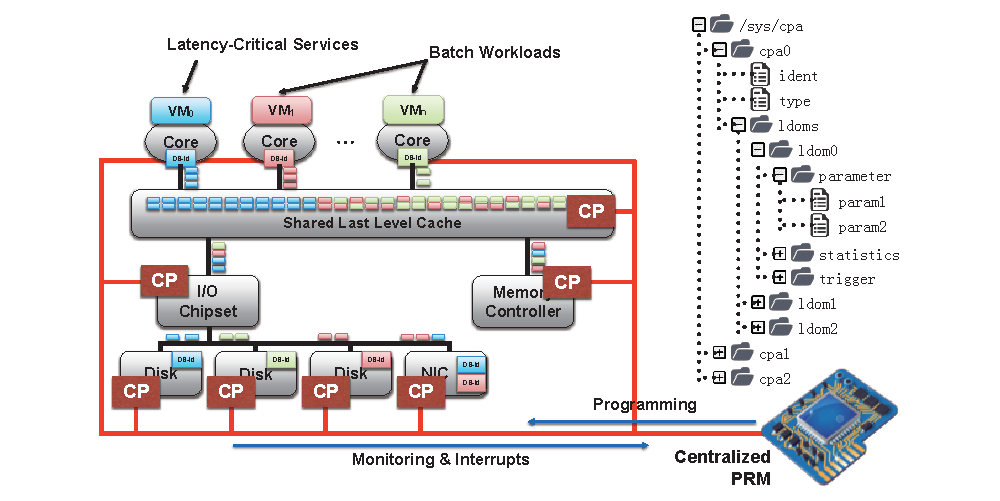
\includegraphics{arch/pard-arch-outline.pdf}
  \caption[PARD体系结构概况]{PARD体系结构概况}
  \label{fig:pard-arch-outline}
\end{figure}

